\chapter{Theoretische Grundlagen}
\label{sec:t_grund}
Die Waitinglist soll nicht ersetzt, sondern die Waitinglist-Bearbeiter entlastet werden.  
Daher soll das Modell nicht nur Vorhersagen über das Ereignis treffen, sondern auch die Wahrscheinlichkeit angeben, mit der ein bestimmtes Ergebnis eintritt.  
So erhalten die Bearbeiter eine Einschätzung darüber, wie sicher das Modell bei seiner Vorhersage ist.

Ein Beispiel wäre, dass eine Buchung zu $90\%$ Wahrscheinlichkeit von der Waitinglist angenommen wird. 
Der Bearbeiter kann also mit hoher Sicherheit nach kurzer Überprüfung die Buchung annehmen.
Um die Entlastung weiter zu erhöhen, könnte die Annahme oder Ablehnung einer Buchung automatisch von der Waitinglist verarbeitet werden, sobald ein bestimmter Schwellwert, beispielsweise $90\%$, erreicht wird.

Für die Vorhersage gibt es zwei grundlegende Ansätze: Regression und Klassifikation.  
Während die Regression eine numerische (quantitative) Zielgröße vorhersagt, bestimmt die Klassifikation eine kategoriale (qualitative) Zielgröße, die als Klassenlabel bezeichnet wird \parencite[95]{vonderHude2020}.

In diesem Fall wird eine Wahrscheinlichkeit für die Entscheidung auf der Waitinglist benötigt, wodurch sich das Problem als Klassifikationsaufgabe einordnen lässt.  
Da genau zwei mögliche Ergebnis-Kategorien existieren (\enquote{Annahme} oder \enquote{Ablehnung}), handelt es sich um ein binäres Klassifikationsproblem.

\section{Datenbanktheorie}
Um einen Datensatz aus einer Datenbank zu aggregieren, benötigt man eine Grundlage der Datenbanktheorie.
Es gibt verschiedene Datenbanktypen, in der Arbeit geht es alleine um relationale SQL-Datenbanken.

Dies bedeutet, dass Daten in Tabellen mit festen Spalten gespeichert werden und über Relationen miteinander verknüpft sind \cite{Elmasri2015}. Jede Tabelle besitzt Attribute, die bestimmte Eigenschaften der gespeicherten Entitäten repräsentieren. Zur eindeutigen Identifikation eines Datensatzes kann eine Tabelle einen \enquote{Primärschlüssel} enthalten, beispielsweise eine eindeutige Identifikationsnummer.  


Mit einem \lstinline[language=SQL]|SELECT|-Statement können gezielt Datensätze aus einer Tabelle abgefragt werden. Ein solches Statement besteht grundlegend aus drei Hauptkomponenten:  
\begin{enumerate}[noitemsep]
    \item Den ausgewählten Attributen, die zurückgegeben werden sollen
    \item Der angegebenen Tabelle, aus der die Daten stammen 
    \item Der \lstinline[language=SQL]|WHERE|-Klausel, in der Bedingungen für die Selektion definiert werden können. 
\end{enumerate}

Beispielsweise kann in einer Tabelle mit Schiffsdatensätzen gezielt nach einem Schiff mit einer bestimmten Nummer gesucht werden:
\begin{lstlisting}[language=SQL]
SELECT * FROM Schiffe WHERE schiffsnummer = 12345;
\end{lstlisting}

\paragraph{JOIN}
Häufig stehen Tabellen in einer relationalen Datenbank in Beziehung zueinander. Dabei gibt es verschiedene Arten von Relationen:
\begin{itemize}[noitemsep]
    \item 1:1-Beziehung: Jeder Datensatz in der ersten Tabelle ist genau einem Datensatz in einer anderen Tabelle zugeordnet \cite{Elmasri2015}.
    \item 1:n-Beziehung: Ein Datensatz der ersten Tabelle kann mit mehreren Datensätzen in einer anderen Tabelle in Verbindung stehen \cite{Elmasri2015}.
\end{itemize}

Um Daten aus mehreren Tabellen gleichzeitig abzufragen, werden Joins verwendet. Ein \lstinline[language=SQL]|JOIN| ermöglicht es, Tabellen auf Basis gemeinsamer Schlüsselattribute zu verknüpfen und die relevanten Datensätze gemeinsam auszugeben.
Hierfür wird also eine Tabelle angegeben, sowie eine optionale Bedingung, unter der die Spalten miteinander verbunden werden sollen.
Wenn im Beispiel das vorherige Schiff mit einem Besitzer verbunden werden soll, könnte dies so aussehen:
\begin{lstlisting}[language=SQL]
SELECT * FROM Schiffe 
JOIN Besitzer 
ON Besitzer.nummer = Schiffe.besitzernummer
WHERE schiffsnr = 12345;
\end{lstlisting}

Mengentheoretisch betrachtet, führt ein \lstinline[language=SQL]|JOIN|
eine Mengenoperation auf zwei Relationen (Tabellen) durch. Dabei werden Datensätze aus beiden Tabellen anhand eines definierten Schlüssels kombiniert. Dies entspricht dem kartesischen Produkt der beiden Mengen, gefolgt von einer Selektion, die nur die passenden Tupel (Datensätze) gemäß der \lstinline[language=SQL]|JOIN|-Bedingung beibehält \cite{Elmasri2015}.

Pro \lstinline[language=SQL]|JOIN| werden alle Tabelleneinträge beider Tabellen miteinander verbunden, sofern die Join-Bedingung erfüllt ist.  
Sei \( a \) die Anzahl der Zeilen in Tabelle 1 und \( b \) die Anzahl der Zeilen in Tabelle 2, dann ergibt eine \lstinline[language=SQL]|JOIN| Operation maximal \( a \times b \) Ergebniszeilen.  
Diese Anzahl wird durch die \lstinline[language=SQL]|ON| Bedingung reduziert, indem nur jene Kombinationen beibehalten werden, die der definierten Verknüpfungsregel entsprechen.

Ein Beispiel: Eine Tabelle mit $20$ Schiffen wird mit einer Tabelle von $10$ Besitzern gejoint.  
Ohne eine spezifische \lstinline[language=SQL]|ON|-Bedingung würde jedes Schiff mit jedem Besitzer kombiniert, sodass zunächst $20 \times 10 = 200$ Zwischenergebniszeilen entstehen.  

Falls jedoch eine \lstinline[language=SQL]|ON|-Bedingung gesetzt wird, um nur Schiffe mit ihren tatsächlichen Besitzern zu verknüpfen, reduziert sich die Ergebnismenge auf die tatsächlichen $20$ gültigen Zuordnungen.  
Dennoch wirkt sich ein \lstinline[language=SQL]|JOIN| mit großen Tabellen auf die Performance der Abfrage aus. Je mehr Zeilenkombinationen erzeugt werden, umso länger dauert auch die Berechnung.
\paragraph{Datenaggregation mit GROUP BY}

Das \lstinline[language=SQL]|GROUP BY|-Statement wird verwendet, um Daten nach bestimmten Attributen zu gruppieren und aggregierte Werte für jede Gruppe zu berechnen \cite{Elmasri2015}. 
Dies ist besonders nützlich, wenn Informationen über Gruppen von Datensätzen benötigt werden, z. B. die Anzahl der Schiffe pro Besitzer oder der durchschnittliche Containerinhalt pro Hafen.

Dabei sind $2$ Komponenten relevant:
\begin{itemize}[noitemsep]
    \item Attribute, anhand Zeilen gruppiert werden sollen.
    \item Aggregatfunktionen wie \lstinline[language=SQL]|COUNT|, 
    \lstinline[language=SQL]|SUM|, 
    \lstinline[language=SQL]|AVG| 
    oder \lstinline[language=SQL]|MAX|, die angewendet werden sollen.
\end{itemize}
Ein Beispiel zur Ermittlung der Anzahl der Schiffe pro Besitzer:

\begin{lstlisting}[language=SQL]
SELECT besitzernummer, COUNT(besitzernummer) AS anzahl_schiffe
FROM Schiffe
GROUP BY besitzernummer;
\end{lstlisting}

\paragraph{Temporäre Zwischentabellen mit WITH}
Das \lstinline[language=SQL]|WITH|-Statement, auch als \gls{cte} bezeichnet, ist eine Möglichkeit, komplexe SQL-Abfragen übersichtlicher zu gestalten und Zwischenergebnisse in einer Abfrage mehrfach zu verwenden \cite{Horvat2008}.  
Statt eine verschachtelte Unterabfrage direkt in der Hauptabfrage zu definieren, wird eine temporäre Tabelle erstellt, die in der Hauptabfrage referenziert werden kann.
Durch die Nutzung von \glspl{cte} können lange und verschachtelte Abfragen in kleinere, verständliche Teile aufgeteilt werden:
\begin{lstlisting}[language=SQL]
WITH Zwischentabelle AS (
    [...]
) 
SELECT [...]
FROM Zwischentabelle
\end{lstlisting}

Des Weiteren können Teile einer Query stufenweise ausgeführt werden, um Zwischenergebnismengen zu reduzieren.
Die Kombination aus \lstinline[language=SQL]|WITH| und 
\lstinline[language=SQL]|GROUP BY|
kann also verwendet werden, um zwischen verschiedenen \lstinline[language=SQL]|JOIN|-Statements eine Gruppierung durchzuführen.

\section{Eingesetzte Algorithmen des maschinellen Lernens}

Bei maschinellen Lernalgorithmen lässt sich grundsätzlich zwischen regelbasierten und statistischen Algorithmen unterscheiden.
Regelbasierte Algorithmen nutzen vordefinierte Entscheidungslogiken, während statistische Algorithmen datengetriebene Optimierungen berechnen \cite{RussellNorvig2020}. 
Für die Auswahl der \gls{ml}-Modelle kommen keine regelbasierten Algorithmen infrage, da von \gls{hl} keinen festen Regeln definiert werden können.
Daher sind nur statistische \gls{ml}-Algorithmen für das Problem anwendbar. 

Die \gls{ml}-Modelle können entweder überwacht (supervised) oder unüberwacht (unsupervised) lernen. 
Beim überwachten Lernen erhält ein Modell gelabelte Daten (Eingabe-Ausgabe-Paare).
Hingegeben beim unüberwachten Lernen werden nur die Eingabe-Parameter übergeben \cite{Goodfellow2016}.

Die Modelle für die Waitinglist-Vorhersagen sollen basierend auf den vergangenen Entscheidungen trainiert werden. 
Es sind also Eingabe-Ausgabe-Paare vorhanden und daher wird überwacht trainiert.

\pagebreak
Für das überwachte Lernen werden die folgenden \gls{ml}-Algorithmen implementiert:
\begin{itemize}
    \item \textbf{Neuronale Netze:}
    Neuronale Netze sind leistungsstarke Modelle, die komplexe, nicht lineare Zusammenhänge in Daten erfassen können.  
    Da es sich bei der Vorhersage von Waitinglist-Entscheidungen um eine binäre Klassifikationsaufgabe handelt, sind neuronale Netze besonders gut geeignet. Sie eignen sich besonders, wenn die Entscheidungsgrenzen nicht linear sind und viele Merkmale eine Rolle spielen.  In früheren Anwendungen haben sich neuronale Netze für binäre Klassifikationen als leistungsfähige Modelle erwiesen, insbesondere wenn die zugrunde liegenden Entscheidungsprozesse nicht durch einfache Regeln beschrieben werden können \cite{LeCun2015}. Sie sind sehr individuell auf ein Problem anpassbar, somit muss die Technik für eine Verwendung gut verstanden werden, um Parameter bei der Implementation festzulegen.
    
    \item \textbf{Entscheidungsbäume und Random Forests:}
    Entscheidungsbäume sind leicht interpretierbare Modelle, die durch rekursive Unterteilung der Daten eine hierarchische Entscheidungsstruktur erzeugen \cite{Breiman2001}.  
    Da sie gut mit nicht linearen Entscheidungsregeln umgehen können und leicht interpretierbar sind, eignen sie sich für die Vorhersage von Waitinglist-Entscheidungen. 
    Allerdings neigen Entscheidungsbäume zum Overfitting, weshalb oft der Random Forest eingesetzt wird.  

    Bei \gls{ml}-Modellen tritt häufig das Problem des Overfittings auf.  
    Overfitting bedeutet, dass ein Modell die Trainingsdaten zu genau lernt, anstatt allgemeine Zusammenhänge zu erfassen \cite{Goodfellow2016}.  
    Dadurch erzielt es auf den Trainingsdaten eine hohe Genauigkeit, zeigt jedoch eine schlechtere Leistung auf neuen, unbekannten Daten, da es nicht gut generalisiert \cite{Bishop2006}.  
    Das ist auch die Bedeutung der Generalisierungsfähigkeit: Ein Modell mit hoher Generalisierungsfähigkeit kann auch auf bislang unbekannten Daten verlässliche Vorhersagen treffen \parencite[110]{Goodfellow2016}.
    
    Random Forest kombiniert mehrere Entscheidungsbäume, um robustere Vorhersagen zu treffen und Overfitting zu reduzieren \cite{Breiman2001}.  
    Dies ist besonders nützlich, wenn viele verschiedene Faktoren die Entscheidung beeinflussen und sich nicht einfach in einer festen Regel zusammenfassen lassen.
    Ein weiterer Vorteil von Entscheidungsbäumen und Random Forest ist die geringe Anzahl an zu bestimmenden Parametern, sowie ihre Ausführungszeit \cite{probst2019hyperparameters}.
    %Hierfür wurde der Random Forest-Algorithmus gewählt. Dieser ist einfacher aufgebaut und braucht weniger Parameter welche bestimmt werden müssen. Dabei ist die Performance (Ausführungszeit) von Random Forest gegenüber Neuronalen Netzen besser.

\pagebreak
    \item \textbf{Logistische Regression:}
    Die logistische Regression ist ein weitverbreitetes Modell für binäre Klassifikationsprobleme \cite{Hastie2009}.  
    Der Name lässt zunächst vermuten, dass es sich ausschließlich um eine Regression handelt.
    Sie basiert auf einer linearen Entscheidungsfunktion, die eine Wahrscheinlichkeit als Ausgabe liefert. 
    Sie eignet sich dadurch auch für binäre Klassifikationsprobleme, da hierbei auch nur eine Wahrscheinlichkeit benötigt wird. 
    Die logistische Regression eignet sich besonders, wenn die Entscheidungsgrenze linear trennbar ist und die Interpretierbarkeit der Vorhersagen eine hohe Relevanz hat.  
    Zudem wird keine umfangreiche Parameterbestimmung, wie bei den neuronalen Netzen, benötigt \cite{Bishop2006}.  
    Ein Nachteil besteht jedoch darin, dass sie mit komplexen, nicht linearen Zusammenhängen in den Daten schlechter umgehen können.  

\end{itemize}


%5.2 Capacity, Overfitting and Underfitting: The ability to perform well on previously unobserved inputs is called generalization.

\subsection{Neuronale Netze}

%1. Allgemin
%1.1 Eingabe Ausgabe
%1.2 Neuron (Aktivierung)
%1.3 Layers Hidden etc
%Backpropergation
% -> Loss Fuction
%Strukturen -> Feed Forewrds
%Aktivierungsfunktion
%Drouput
%


%\todo{IW: Random Forest muss auch so gut erklärt werden}
%Ich habe nichts gegen die ausführliche Erklärung hier einzuwenden. Dann sollten Sie Random Forest aber genau so ausführlich erklären.

Neuronale Netze sind ein wichtiges Teilgebiet im \gls{ml} und werden heute in vielen Bereichen der \gls{ki} eingesetzt \cite{Goodfellow2016}. Sie orientieren sich an der Struktur und Arbeitsweise des menschlichen Gehirns, indem sie eine große Anzahl von Knoten, sogenannte Neuronen, miteinander verknüpfen. Dadurch können sie komplexe Zusammenhänge in Daten erkennen und nutzen \cite{Schmidhuber2015}. Das Hauptziel eines neuronalen Netzes ist es, Eingabedaten in sinnvolle Ausgaben umzuwandeln, wobei das Netzwerk durch Training lernt, diese Transformation schrittweise zu verbessern. 
Also als Beispiel könnten verschiedene Schiffsattribute wie Schiffsbeladung, Fahrtlänge, Windgeschwindigkeit als Eingabedaten in eine Vorhersage transformiert werden, ob ein Containerschiff pünktlich ankommt.

Hierbei kommen mathematische Operationen zum Einsatz, bei denen Gewichte (Weights) und Schwellenwerte (Biases) angepasst werden, um die Ergebnisse zu optimieren \cite{Bishop2006}.

\begin{figure}[H]
    \centering
    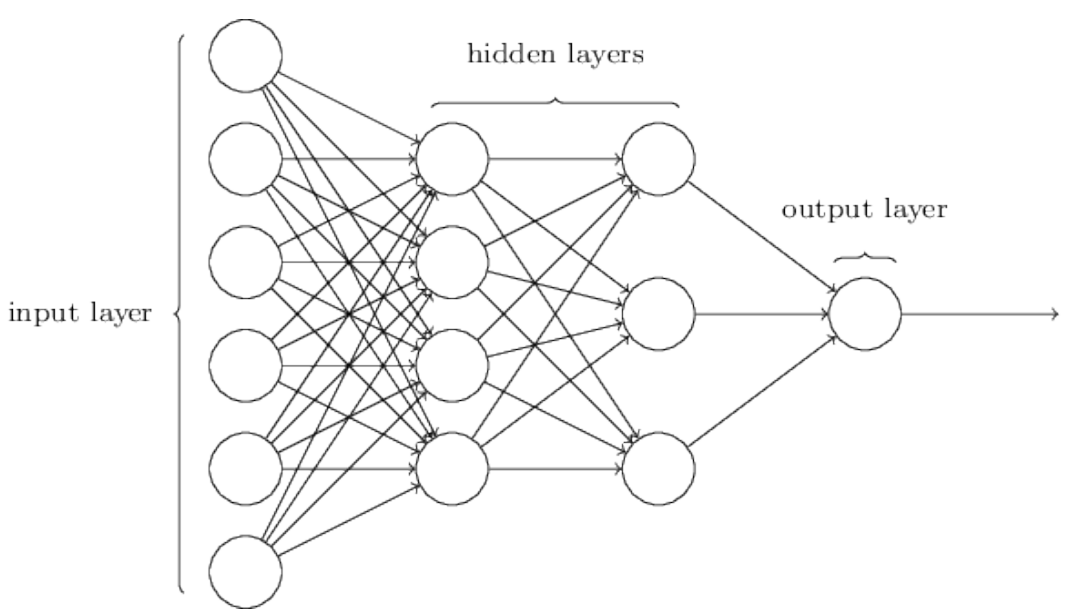
\includegraphics[width=0.8\linewidth]{Thesis//bilder/input_hidden_output_layers.png}
    \caption
    [Schematische Darstellung eines neuronalen Netzes]
    {Schematische Darstellung eines neuronalen Netzes \parencite[11]{nielsen2015neural}}
    \label{fig:neural_net_schema}
\end{figure}

Ein neuronales Netz besteht aus drei Hauptkomponenten: der Eingabeschicht (input layer), den versteckten Schichten (hidden layers) und der Ausgabeschicht (output layer) \cite{nielsen2015neural}. Die Eingabeschicht nimmt die Rohdaten entgegen und gibt sie an die nächsten Schichten weiter. 
Jede Eingabe entspricht dabei einem Merkmal der Daten. 
In den versteckten Schichten, die das Kernstück des Netzwerks bilden, werden diese Daten verarbeitet, um Muster und Strukturen zu erkennen.
Die Ausgabeschicht liefert schließlich das Ergebnis, wie beispielsweise eine Klassifikation.

Die Funktionsweise eines neuronalen Netzes lässt sich in zwei Schritte unterteilen: die Vorwärtspropagierung und die Rückpropagierung \cite{Rumelhart1986}. Bei der Vorwärtspropagierung durchlaufen die Daten das Netzwerk von der Eingabeschicht über die versteckten Schichten bis zur Ausgabeschicht. In jedem Neuron werden die Eingaben gewichtet, summiert und durch eine Aktivierungsfunktion transformiert, bevor sie an die nächste Schicht weitergegeben werden. Während des Trainingsprozesses erfolgt dann die Rückpropagierung, bei der die Gewichte des Netzwerks angepasst werden, um den Fehler zu minimieren. Dies geschieht in der Regel mithilfe des Gradientenabstiegs \cite{Kingma2015}.

Ein entscheidender Bestandteil eines neuronalen Netzes sind die Aktivierungsfunktionen, die für die Einführung von Nichtlinearität sorgen \cite{Goodfellow2016}. Ohne diese Nichtlinearität würde das Netzwerk lediglich eine lineare Transformation der Eingaben durchführen und hätte damit die gleiche Ausdrucksstärke wie ein einfaches lineares Modell \cite{Goodfellow2016}. %Goodfellow2016: Seite 172

%\todo{IW: Quatsch??!?!?!?}
%Ich sehe hier keinen Zusammenhang zu den komplexen Mustern: Wo haben Sie denn das gelesen?
%Eine nichtlineare Aktivierungsfunktion sorgt vor allem dafür, dass nicht alle Beispiele voll durchschlagen und das Netz beim Lernen hin- und herspringt.

%Aktivierungsfunktionen

Das Training eines neuronalen Netzes läuft in mehreren Schritten ab. Zunächst werden die Gewichte und Schwellenwerte zufällig initialisiert. Anschließend durchlaufen die Trainings-Eingabedaten das Netzwerk, und die Vorhersagen werden berechnet (Forward Pass). Danach wird der Fehler (Loss) mit einer Fehlerfunktion (Loss Function) ermittelt \cite{Goodfellow2016}. Mithilfe der Rückpropagierung werden die Gewichte so angepasst, dass der Fehler nach und nach minimiert wird.

\subsubsection{Rückpropagierung}
Die Rückpropagierung (Backpropagation) ist ein essenzieller Mechanismus, der das Lernen in neuronalen Netzen ermöglicht. Sie basiert auf einem schrittweisen Anpassungsprozess der Gewichte und Biases des Netzwerks, um die Diskrepanz zwischen der vorhergesagten und der tatsächlichen Ausgabe zu minimieren. Der Prozess kann in vier Phasen unterteilt werden:

\begin{enumerate}
    \item \textbf{Fehlerberechnung:} \\
    Nach der Vorwärtspropagierung wird die Differenz zwischen der vorhergesagten und der tatsächlichen Ausgabe berechnet. Diese Differenz wird durch eine Fehlerfunktion (Loss Function) wie den Mean Squared Error (MSE) oder die Cross-Entropy quantifiziert \cite{Goodfellow2016, Schmidhuber2015}. (Siehe \ref{sec:lossfunction})

    \item \textbf{Berechnung der Gradienten:} \\
    Mithilfe der Kettenregel wird der Gradient der Fehlerfunktion nach den Gewichten berechnet. Der Gradient gibt an, wie stark eine Änderung der Gewichte den Fehler beeinflusst. Diese Berechnung erfolgt schichtweise rückwärts, beginnend bei der Ausgabeschicht bis hin zur Eingabeschicht \cite{Rumelhart1986}.
    
    \item \textbf{Gewichtsaktualisierung:} \\
    Die Gewichte werden mithilfe einer Optimierungsstrategie wie dem Gradientenabstieg aktualisiert. Dabei werden die Gewichte proportional zum berechneten Gradienten angepasst, um den Fehler zu reduzieren. Die Größe der Anpassung wird durch die Lernrate (Learning Rate) gesteuert \cite{Kingma2015}.
    
    \item \textbf{Iterative Wiederholung:} \\
    Dieser Prozess wird für alle Trainingsdaten wiederholt. Jede Iteration wird als Epoche bezeichnet. Das Ziel ist es, den Fehler über alle Trainingsbeispiele hinweg zu minimieren, sodass das Netzwerk in der Lage ist, verallgemeinerte Muster zu lernen \cite{nielsen2015neural}.
\end{enumerate}

Die Rückpropagierung ist somit der Kern des Trainingsprozesses in neuronalen Netzen. Sie ermöglicht es, dass die Gewichte und Biases des Netzwerks so angepasst werden, dass das Netzwerk zunehmend genauere Vorhersagen treffen kann \cite{LeCun2015}

\subsubsection{Fehlerfunktion}
\label{sec:lossfunction}
Bei der Vorwärtspropagierung wird mittels der Fehlerfunktion die Differenz zwischen der vorhergesagten und der tatsächlichen Ausgabe berechnet. Ziel des Trainings ist es, diese Differenz, auch als Fehler bezeichnet, zu minimieren, indem die Gewichte des Netzwerks iterativ angepasst werden \cite{Goodfellow2016}.

Es gibt verschiedene Fehlerfunktionen, die für unterschiedliche Arten von Problemen verwendet werden.
Bei einer Regressionsaufgabe, bei der ein Modell kontinuierliche Werte vorhersagen soll, wird häufig der \gls{mse} genutzt \cite{Goodfellow2016}. 
Diese Fehlerfunktion berechnet den Durchschnitt der quadrierten Abweichungen zwischen den vorhergesagten und den tatsächlichen Werten. Durch das Quadrieren werden größere Fehler stärker bestraft, wodurch das Modell genauer an die tatsächlichen Werte angepasst wird.

Bei einem Klassifikationsproblem, bei dem eine Eingabe einer bestimmten Kategorie zugeordnet werden soll (z.B. \enquote{Annahme} oder \enquote{Ablehnung}), ist die Cross-Entropy eine geeignete Wahl. Diese Fehlerfunktion misst, wie gut die vorhergesagte Wahrscheinlichkeitsverteilung mit der tatsächlichen übereinstimmt.

Ein wichtiger Vorteil der Cross-Entropy gegenüber dem \gls{mse} für Klassifikationsaufgaben liegt in der Art, wie das Modell daraus lernt. Während \gls{mse} die Fehler gleichmäßig gewichtet, sorgt die Cross-Entropy dafür, dass große Unsicherheiten stärkere Korrekturen erhalten \cite{Goodfellow2016}.

Für binäre Klassifikationsprobleme gibt es die \gls{bce}, welche insbesondere für Probleme mit nur zwei möglichen Klassen eingesetzt wird. Die \gls{bce} berechnet den Fehler basierend auf der Differenz zwischen den vorhergesagten Wahrscheinlichkeiten und den tatsächlichen Klassenzugehörigkeiten und wird oft in Kombination mit der Sigmoid-Aktivierungsfunktion genutzt.

Eine Erweiterung der \gls{bce} ist die sogenannte \enquote{Binary Cross-Entropy with Logits}, die eine numerisch stabilere Berechnung ermöglicht, indem die Sigmoid-Funktion direkt in die Fehlerberechnung integriert wird \cite{Goodfellow2016}. 
Diese Methode verbessert die Stabilität des Trainings, da separate Berechnungen der Sigmoid-Aktivierung und der Cross-Entropy zu numerischen Ungenauigkeiten führen können. Zusätzlich kann diese Funktion gewichtet werden, um Klassenungleichgewichte im Datensatz zu berücksichtigen. Dabei werden unterrepräsentierte Klassen stärker gewichtet, um sicherzustellen, dass das Modell auch diese Klassen effektiv lernt. Dies ist besonders wichtig in Datensätzen mit stark unausgeglichenen Klassen, da ansonsten die Minderheitsklasse vom Modell vernachlässigt werden könnte \cite{Hastie2009}.

\subsubsection{Modellstrukturen}
Die Struktur eines neuronalen Netzes kann auf viele verschiedene Weisen aufgebaut werden. 
Die grundlegende Struktur eines neuronalen Netzes wird durch die Anzahl der Schichten, die Anzahl der Neuronen pro Schicht sowie die Art der Verbindungen zwischen den Schichten bestimmt \cite{Goodfellow2016}. 
Die Wahl der Modellstruktur beeinflusst maßgeblich die Lernfähigkeit, Rechenkomplexität und Generalisierungsfähigkeit des Netzwerks \cite{LeCun2015}.  

Für binäre Klassifikationsprobleme bieten sich Feedforward-Netze an. Diese Netzwerke bestehen aus einer Abfolge von Schichten, bei denen die Ausgabe einer Schicht als Eingabe für die nächste Schicht dient \cite{nielsen2015neural}. Laut Wong et al. \cite{wong2011comparing} zeigen Feedforward-Netze zuverlässige Ergebnisse und sind durch ihre einfache Struktur und Flexibilität eine bevorzugte Wahl für solche Aufgaben.

Bei der Struktur eines Feedforward-Netzes müssen zahlreiche Entscheidungen getroffen werden, die maßgeblich die Leistungsfähigkeit des Modells beeinflussen. Dazu gehören unter anderem:
\begin{itemize}[noitemsep]
    \item \textbf{Anzahl der versteckten Schichten (hidden layers):}  
    Die Anzahl der Schichten bestimmt die Tiefe des Netzwerks. Mehr Schichten ermöglichen es, komplexere Muster zu lernen, können aber auch die Gefahr von Overfitting erhöhen \cite{Goodfellow2016}.
    \item \textbf{Anzahl der Neuronen pro Schicht:}  
    Die Anzahl der Neuronen in einer Schicht beeinflusst zusammen mit der Anzahl der Schichten die Kapazität des Netzwerks, komplexe Muster in den Daten zu lernen. Eine Erhöhung der Neuronenanzahl hat einen ähnlichen Effekt wie das Hinzufügen zusätzlicher Schichten: Das Netzwerk wird leistungsfähiger und kann detailliertere Zusammenhänge in den Daten modellieren. Gleichzeitig steigt jedoch das Risiko von Overfitting, da das Netzwerk in der Lage sein könnte, nicht nur die relevanten Muster, sondern auch zufällige Abweichungen (Rauschen) in den Trainingsdaten zu lernen \cite{Goodfellow2016}.
    \item \textbf{Aufbau der Schichten:}  
    Der Aufbau umfasst die Reihenfolge und die Art der Schichten. Dabei ist gemeint, dass pro Schicht die Aktivierungsfunktion und, falls gewollt, weitere Komponenten in eine Schicht eingepflegt werden können, um die Generalisierungsfähigkeit und Lernfähigkeit zu steigern \cite{Goodfellow2016}.
\end{itemize}


\subsubsection{Aktivierungsfunktionen}
Zu den bekanntesten Aktivierungsfunktionen zählt die Sigmoid-Funktion, die hohe Eingabewerte in Richtung $1$ und niedrige Werte in Richtung $0$ transformiert und sich daher gut zur Darstellung von Wahrscheinlichkeiten eignet \cite{Hastie2009}.  
Ebenso häufig verwendet wird die \acrshort{relu}-Funktion (\acrlong{relu}), die negative Werte auf $0$ setzt, während positive Werte unverändert bleiben.

\begin{figure}[H]
    \centering
    \begin{subfigure}[b]{0.32\textwidth}
        \centering
        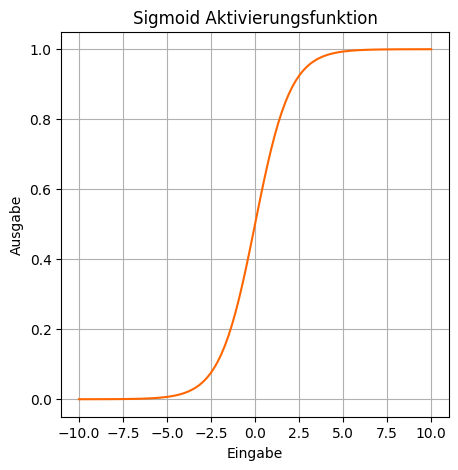
\includegraphics[width=\linewidth]{Thesis/bilder/Sigmoid-G.png}
    \end{subfigure}
%    \begin{subfigure}[b]{0.2405\textwidth}
%        \centering
%        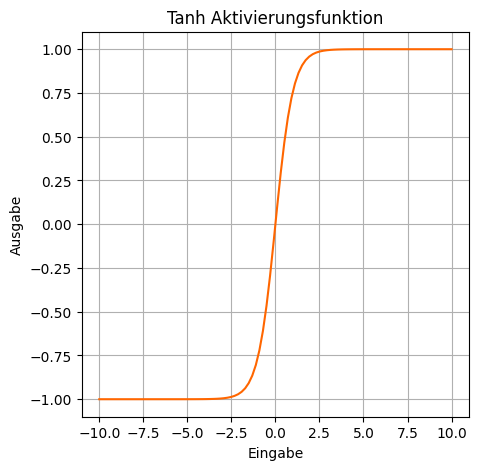
\includegraphics[width=\linewidth]{Thesis/bilder/TanH-G.png}
%    \end{subfigure}
    \begin{subfigure}[b]{0.32\textwidth}
        \centering
        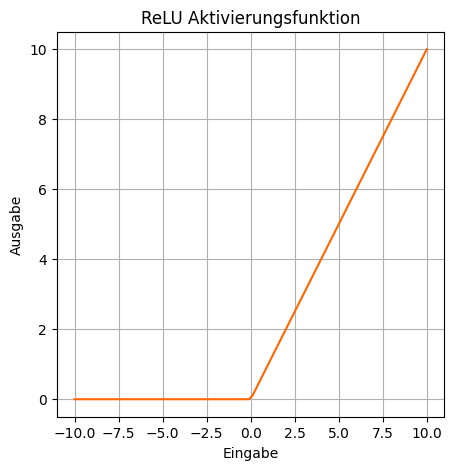
\includegraphics[width=\linewidth]{Thesis/bilder/ReLU-G.png}
    \end{subfigure}
    \begin{subfigure}[b]{0.32\textwidth}
        \centering
        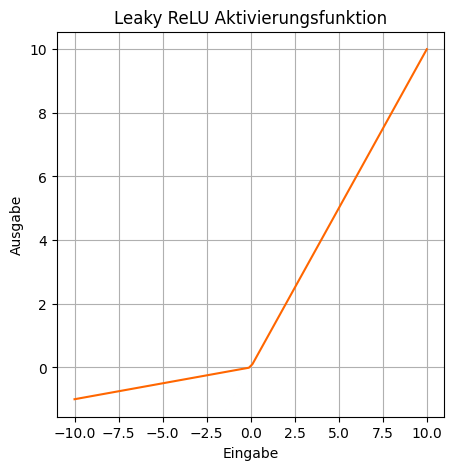
\includegraphics[width=\linewidth]{Thesis/bilder/LeakyReLU-G.png}
    \end{subfigure}
    \caption{Visualisierung der Aktivierungsfunktionen Sigmoid, \acrshort{relu} und Leaky\acrshort{relu}}
\end{figure}

Ein entscheidender Vorteil von \gls{relu} gegenüber Sigmoid ist die Vermeidung des \enquote{Vanishing Gradient Problems}. Dieses Problem tritt auf, wenn Aktivierungsfunktionen mit flachen Ableitungen, wie die Sigmoid-Funktion, verwendet werden. Da deren Ableitungen für große oder kleine Werte nahe $0$ sind, werden die Gradienten in tiefen Netzwerken während der Rückpropagierung zunehmend kleiner. Da die Gewichtsanpassung beim Gradientenabstieg proportional zur Ableitung der Aktivierungsfunktion ist, führt dies dazu, dass die frühen Schichten des Netzes nur noch sehr langsam oder gar nicht mehr lernen \cite{Goodfellow2016}.

\gls{relu} vermeidet dieses Problem, indem es für positive Werte eine konstante Ableitung von 1 besitzt. Die Eigenschaft, dass negative Werte auf 0 gesetzt werden, sorgt für eine sparsame Aktivierung, wodurch einige Neuronen inaktiv bleiben und Overfitting reduziert werden kann \cite{Goodfellow2016}.


\begin{wrapfigure}[10]{r}{0.6\textwidth}
    \centering
    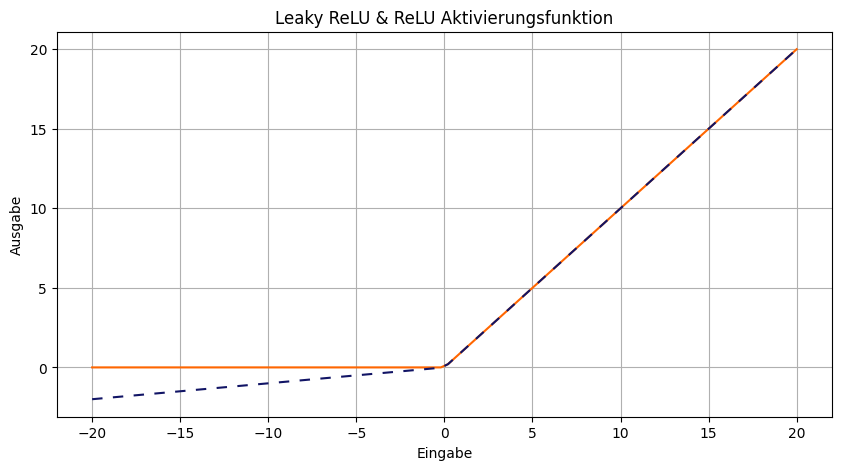
\includegraphics[width=\linewidth]{Thesis//bilder/ReLUVergleich.png}
    \caption{\gls{relu} und Leaky-\gls{relu} Visualisierung}
    \label{fig:relu_leaky_relu}
\end{wrapfigure}



Als Alternative zur \gls{relu}-Funktion kann die Leaky\gls{relu}-Funktion verwendet werden.
Bei Leaky\acrshort{relu} sind die negativen Eingabewerte nicht vollständig auf 0 gesetzt, sondern werden mit einem kleinen Faktor multipliziert, um das sogenannte \enquote{Dead Neurons}-Problem zu reduzieren. 

Das \enquote{Dead Neurons Problem} tritt auf, wenn ein Neuron durch eine Aktivierungsfunktion wie \gls{relu} ständig einen Ausgangswert von 0 liefert.  
Da die Ableitung der \gls{relu}-Funktion für negative Werte ebenfalls 0 ist, bedeutet dies, dass das Neuron im Rückpropagierung-Prozess keine Gewichtsaktualisierung mehr erhält und somit effektiv „tot“ bleibt \cite{Glorot2011}.  

Bei tiefen neuronalen Netzen kann dieses Problem dazu führen, dass ein erheblicher Teil der Neuronen keine Lernfähigkeit mehr besitzt, was die Modellleistung beeinträchtigen kann \cite{Goodfellow2016}.
Ob die Leaky-\gls{relu}-Funktion eine Verbesserung bringt und daher verwendet werden sollte, kann durch experimentelles Testen bestimmt werden.

\subsubsection{Weitere Komponenten}
Um das Overfitting zu vermeiden, die Stabilität und die Generalisierungsfähigkeit zu steigern, können weitere Komponenten in ein Modell eingesetzt werden. 
In dieser Arbeit werden zwei Techniken verwendet: Dropout und Batch-Normalisierung.

\paragraph{Dropout}
Die Trainingsdaten werden durch mehrere Epochen mehrmals in ein Netz zum Training eingegeben. Hierbei werden zufällig Neuronen deaktiviert, was verhindert, dass sich das Modell zu stark auf spezifische Muster in den Trainingsdaten konzentriert \cite{Srivastava2014}. 
Dieses Verfahren ist besonders bei tiefen Netzwerken wichtig, da diese anfälliger für Overfitting sind.
Hierbei entsteht der neue Parameter \enquote{Dropout-Rate}. 
Dieser gibt an, wie viel Prozent der Neuronen deaktiviert werden sollen. 

\pagebreak
\paragraph{Batch-Normalisierung}
Batch-Normalisierung ist eine Technik zur Stabilisierung und Beschleunigung des Trainings neuronaler Netze, indem sie die Aktivierungen einer Schicht normalisiert \cite{Ioffe2015}.  
Dabei werden die Eingaben einer Schicht auf einen Mittelwert von 0 und eine feste Standardabweichung skaliert.  

Batch-Normalisierung adressiert insbesondere das \enquote{Internal Covariate Shift Problem}, das auftritt, wenn sich die Verteilung der Aktivierungen innerhalb des Netzwerks während des Trainings kontinuierlich verändert.  
Da die Gewichte eines neuronalen Netzes in jeder Iteration angepasst werden, verändern sich auch die Eingangsverteilungen der nachfolgenden Schichten fortlaufend. Dies erschwert das Training, da sich jede Schicht wiederholt an neue Verteilungen anpassen muss, was zu instabilen Gradienten, langsameren Lernraten und längeren Konvergenzzeiten führt \cite{Ioffe2015}.  
Die Konvergenzzeit bezeichnet die Dauer, die ein Modell benötigt, um eine stabile Lösung oder ein Optimum zu erreichen.


Als Beispiel nehmen wir an, dass die Aktivierungen einer Schicht, Werte im Bereich von $-100$ bis $200$ annehmen, während eine andere Schicht nur Werte zwischen $-1$ und $1$ liefert.  
Diese Unterschiede erschweren das Training, da große Aktivierungswerte zu übermäßig großen Gradienten führen können, während geringe Werte nur minimale Gewichtsaktualisierungen verursachen.  
Dadurch lernen einige Neuronen schneller als andere, was zu einem instabilen Trainingsprozess führt.  

Batch-Normalisierung skaliert die Aktivierungen jeder Schicht auf eine einheitliche Skala (z. B. Mittelwert 0 und Standardabweichung 1).  
Dies stellt sicher, dass alle Schichten vergleichbare Wertebereiche haben und die Verteilungen über das gesamte Training hinweg stabil bleiben, was zu einem effizienteren und robusteren Lernprozess führt \cite{Ioffe2015}.

\subsection{Random Forest}
%\todo{IW: Genau so ausführlich wie NN}
%Das könnten Sie ruhig genau so ausführlich wie die neuronalen Netze erklären, denn so sagt das keinem etwas, der damit noch nicht gearbeitet hat.

Random Forest ist auch ein Algorithmus des \gls{ml}, der sowohl für Klassifikations- als auch Regressionsaufgaben eingesetzt werden kann \cite{Breiman2001}. Der Algorithmus basiert auf sogenannten Entscheidungsbäumen, um Vorhersagen aus Daten abzuleiten. 

Ein Entscheidungsbaum ist ein hierarchisches Modell, das auf einer Folge von Ja/Nein-Entscheidungen basiert und eine Eingabe durch schrittweise Abfragen auf eine bestimmte Klasse oder einen numerischen Wert zuordnet \cite{Breiman2001}.  
Jeder Knoten im Baum stellt eine Bedingung für ein Merkmal dar (z. B. \enquote{Ist das Gewicht der Container größer als 10 Tonnen?}), während die Blätter des Baums die endgültige Vorhersage enthalten.  
 
Das Training eines Entscheidungsbaums geschieht in mehreren Schritten:

\begin{enumerate}[noitemsep]
    \item \textbf{Wahl des besten Splits:}  
    Der Algorithmus wählt das Merkmal und den Schwellenwert, mit dem die Trainingsdaten am besten getrennt werden.  
    Dies wird durch ein Maß wie dem Gini-Index bestimmt \cite{5994250}. (Siehe \ref{sec:rf_gini_split})
    \item \textbf{Rekursive Teilung:}  
    Nach dem ersten Split wird der gleiche Vorgang rekursiv auf die entstandenen Teilmengen angewendet, bis ein Abbruchkriterium erreicht ist.
    \item \textbf{Endgültige Klassifikation:}  
    Sobald der Baum nicht weiter aufgeteilt wird, enthalten die Blätter des Baums eine finale Vorhersage.
\end{enumerate}

\subsubsection{Auswahl des besten Splits}
\label{sec:rf_gini_split}
Ein zentraler Schritt im Training eines Entscheidungsbaums ist die Wahl des optimalen Splits an jedem Knoten.  
Dabei wird für jedes Merkmal ein Schwellenwert gesucht, der die Daten am besten trennt.  
Hierzu wird häufig der Gini-Index als Kriterium verwendet.

Der Gini-Index misst die \enquote{Reinheit} einer Gruppe von Datenpunkten.  
Er ist definiert als:

\[
Gini = 1 - \sum_{i=1}^{k} p_i^2
\]

wobei \(p_i\) der Anteil der Klasse \(i\) in der betrachteten Gruppe ist und \(k\) die Anzahl der Klassen angibt.  
Ein Gini-Wert von 0 bedeutet, dass die Gruppe perfekt getrennt ist (alle Punkte gehören zur gleichen Klasse), während ein höherer Wert auf eine höhere Durchmischung hindeutet \cite{5994250}.

\pagebreak
\paragraph{Beispiel: Gini-Index für einen Split}

Angenommen, es existiert einen Datensatz mit Buchungen, die entweder \enquote{angenommen} oder \enquote{abgelehnt} wurden.  
Betrachten wir ein mögliches Merkmal Containergewicht, das zur Trennung der Daten verwendet werden könnte:

\begin{table}[H]
    \centering
    \begin{tabular}{c|c}
        \hline\hline
        \thead{\textbf{Containergewicht (Tonnen)}} & \textbf{Ergebnis} \\
        \hline
        5 & Annahme \\
        7 & Annahme \\
        12 & Annahme \\
        15 & Ablehnung \\
        18 & Ablehnung \\
        \hline\hline
    \end{tabular}
    \caption{Beispieldatensatz für einen Entscheidungsbaum-Split}
    \label{tab:gini-example}
\end{table}

Es würden jetzt alle Schwellwerte, die als Trennpunkte verwendet werden können, getestet. 
Ein möglicher Trennpunkt könnte bei $7$ Tonnen liegen. Dadurch entstehen zwei Gruppen:

\begin{table}[H]
    \centering
    \begin{tabular}{c|cc|c}
        \hline\hline
        \thead{\textbf{Seite}} & \textbf{Annahmen} & \textbf{Ablehnungen} & \textbf{Gini-Index} \\
        \hline
        Links (Gewicht < $7$ Tonnen) & 2 & 0 & $1 - ((2/2)^2 + (0/2)^2) = 0$\\
        Rechts (Gewicht $\ge$ $7$ Tonnen) & 1 & 2 & $1 - ( (1/3)^2 + (2/3)^2 ) = 0\text{,}44$\\
        \hline\hline
    \end{tabular}
    \caption{Beispielsplit mit 7 Tonnen als Schwellwert}
\end{table}

Die Gesamtreinheit des Splits wird durch den gewichteten Durchschnitt berechnet:

\[
Gini_{split} = \frac{2}{5} \times 0 + \frac{3}{5} \times 0\text{,}44 = 0\text{,}264
\]

Wird stattdessen ein anderer Trennpunkt getestet (z. B. $12$ Tonnen), würde sich ein geringerer Gini-Index von $0$ ergeben, was zu einer besseren Trennung führt.

\pagebreak
\subsubsection{Rekursive Aufteilung und Stopp-Kriterien}

Der Algorithmus wählt für jeden Knoten den besten Split und setzt die Aufteilung rekursiv fort, bis eine der folgenden Bedingungen eintritt \cite{5994250}:
\begin{itemize}[noitemsep]
    \item \textbf{Alle Datenpunkte in einem Knoten gehören zur gleichen Klasse (reiner Knoten).}  
    Das Splitting stoppt, wenn der Gini-Index eines Knotens null ist, da dies bedeutet, dass alle enthaltenen Datenpunkte vollständig klassifiziert wurden \cite{5994250}.
    
    \item \textbf{Zu wenige verbleibende Datenpunkte.}  
    Der Entscheidungsbaum hört auf zu wachsen, wenn die Anzahl der Datenpunkte in einem Knoten zu gering ist, um eine sinnvolle Trennung durchzuführen \cite{5994250}.
    
    \item \textbf{Maximale Baumtiefe erreicht.}  
    In vielen Implementierungen wird eine maximale Tiefe des Baums vorgegeben, um Überanpassung an die Trainingsdaten zu verhindern \cite{5994250}.
\end{itemize}


\subsubsection{Verbesserung durch Random Forest}

Obwohl Entscheidungsbäume leistungsfähige Modelle sein können, haben sie zwei zentrale Schwächen:  
\begin{itemize}[noitemsep]
    \item Einzelne Entscheidungsbäume neigen zu Overfitting, wenn sie zu tief wachsen und sich zu stark an die Trainingsdaten anpassen.
    \item Sie sind empfindlich gegenüber kleinen Änderungen in den Daten, da eine kleine Änderung eines Merkmals die gesamte Baumstruktur verändern kann.
\end{itemize}


Random Forest verbessert diesen Ansatz, indem er viele Entscheidungsbäume zu einem sogenannten Ensemble-Modell kombiniert. Jeder Baum trifft eigenständige Vorhersagen, die anschließend aggregiert werden, um die Gesamtvorhersage zu bestimmen.
\begin{figure}[H]
    \centering
    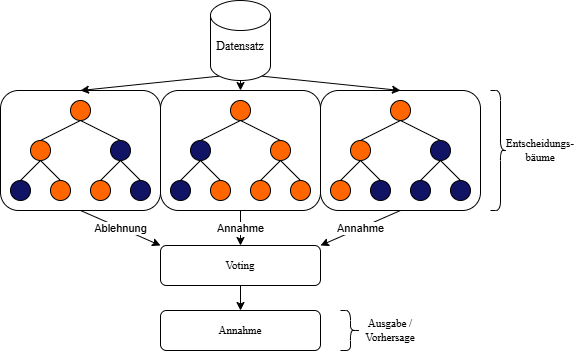
\includegraphics[width=0.5\linewidth]{Thesis//bilder/RF.drawio.png}
    \caption{Beispiel einer Random Forest Vorhersage}
    \label{fig:rf-example}
\end{figure}
Dieses Verfahren führt zu robusteren und genaueren Ergebnissen im Vergleich zu einem einzelnen Baum.


Die Funktionsweise von Random Forest lässt sich in drei wesentliche Schritte unterteilen:
\begin{enumerate}
    \item \textbf{Erstellung von Bootstrap-Stichproben:}  
    Aus den Trainingsdaten werden zufällige Teilmengen mit Zurücklegen gezogen, sodass jeder Entscheidungsbaum eine unterschiedliche Auswahl an Daten sieht \cite{Efron1979}.
    
    \item \textbf{Aufbau der Entscheidungsbäume:}  
    Während des Trainings wird an jedem Knoten eines Baumes nur eine zufällige Teilmenge der Merkmale betrachtet. Dies bedeutet, dass der Algorithmus nicht jedes Merkmal berücksichtigt, sondern für jeden Baum eine andere Auswahl trifft. Dadurch entsteht eine Diversifizierung der Entscheidungsbäume \cite{Ho1995}.
    
    \item \textbf{Aggregierung der Ergebnisse:}  
    Nach dem Training werden die Vorhersagen der einzelnen Bäume kombiniert. Bei Klassifikationsproblemen entscheidet die Mehrheit der Bäume (\enquote{Voting}), während bei Regressionsproblemen der Durchschnitt der Vorhersagen gebildet wird \cite{Breiman2001}.
\end{enumerate}

\subsubsection{Vorteile}
Ein wesentlicher Vorteil von Random Forest zu Entscheidungsbäumen ist seine Robustheit gegenüber Rauschen in den Daten. Durch die Kombination vieler Bäume werden einzelne Fehler ausgeglichen, was zu stabileren Ergebnissen führt. 

Die Implementation ist im Vergleich zu neuronalen Netzen deutlich einfacher, da kaum Parameter festgelegt werden müssen und somit die Implementation nahezu komplett von Softwarebibliotheken übernommen werden kann. Das sorgt auch dafür, dass ein weniger tieferes Verständnis für die Verwendung vom Random Forest-Algorithmus benötigt wird.

%\todo{J: Kannst vielleicht noch mehr zu Feature Importance schreiben. Da gabs auch ein Teil zu, in der Presi von Arnuth}

%\todo{IW: Warum NUR?}
%Warum "nur"?
%Offenbar scheint die Random-Forest-Technik doch das Mittel der Wahl für Ihr Problem zu sein?


%\todo{IW: NN vergleich}
%Wird die Implementierung des neuronalen Netzes denn nicht auch von einer Bibliothek übernommen?

%Vielleicht noch was zu overfitting erklären?
\subsection{Logistische Regression}
Die logistische Regression ist ein Algorithmus des \gls{ml}, der zur Klassifikation von Daten verwendet wird. Sie wird häufig für binäre Klassifikationsprobleme eingesetzt, bei denen eine Entscheidung zwischen zwei möglichen Kategorien getroffen werden muss \cite{Hastie2009}. Im Gegensatz zur linearen Regression, die kontinuierliche Werte vorhersagt, gibt die logistische Regression eine Wahrscheinlichkeit für die Zugehörigkeit zu einer bestimmten Klasse aus.

Die logistische Regression basiert auf der Idee, dass verschiedene Merkmale eines Datensatzes unterschiedlich stark zur Entscheidung beitragen. Dazu wird für jedes Merkmal ein Gewicht bestimmt, das ausdrückt, wie stark dieses Merkmal die Wahrscheinlichkeit einer bestimmten Klassenzugehörigkeit beeinflusst. 

Zunächst berechnet das Modell eine gewichtete Summe aller Merkmale:

\[
z = w_0 + w_1 x_1 + w_2 x_2 + \dots + w_n x_n
\]

Dabei sind \(x_i\) die Werte der Merkmale und \(w_i\) die dazugehörigen Gewichte. \(w_0\) ist der Bias-Wert, der die Grundtendenz der Entscheidung steuert, unabhängig von den Eingabedaten.

Da die berechnete Summe \(z\) theoretisch beliebige Werte annehmen kann, wird sie durch die \textbf{Sigmoid-Funktion} angewendet.
Die Sigmoid-Funktion sorgt dafür, dass sehr große oder sehr kleine Werte von \(z\) in Wahrscheinlichkeiten nahe 1 bzw. 0 umgewandelt werden. Dies macht sie besonders geeignet für Klassifikationsprobleme, bei denen eine Entscheidung auf Basis einer Schwelle (z. B. 0,5) getroffen wird \cite{Bishop2006}. 

Die Modellparameter \(w_i\) werden während des Trainings mithilfe von Optimierungsverfahren angepasst. 
Für die logistische Regression existieren verschiedene numerische Optimierungsverfahren. Minka \cite{Minka2003} vergleicht mehrere Algorithmen hinsichtlich ihrer Effizienz und Konvergenzeigenschaften:

\begin{itemize}[noitemsep]
    \item \textbf{Newton-Verfahren:} Exakte Methode mit schneller Konvergenz, jedoch hoher Rechenaufwand aufgrund der Berechnung der Hesse-Matrix.
    \item \textbf{Konjugierte Gradientenmethode (CG):} Iteratives Verfahren mit guter Konvergenzgeschwindigkeit und effizient für hochdimensionale Daten.
    \item \textbf{Quasi-Newton-Verfahren (BFGS, L-BFGS):} Annäherung an Newton-Verfahren ohne explizite Berechnung der Hesse-Matrix, effizient für große Datensätze.
    \item \textbf{Fixed-Hessian Newton:} Variante der Newton-Methode mit vordefinierter Hesse-Matrix, besonders bei hoch korrelierten Daten vorteilhaft.
    \item \textbf{Iterative Scaling (IS) und Modified Iterative Scaling (MIS):} Früher für Textklassifikation genutzt, jedoch ineffizient im Vergleich zu gradientenbasierten Methoden.
    \item \textbf{Duale Optimierung:} Umformulierung des Problems in den Dualraum, insbesondere für Kernel-Methoden relevant.
\end{itemize}

Es muss also ein Optimierungsverfahren gewählt werden, welches dann die Gewichte \(w_i\) anpasst.
Abgesehen von der Auswahl des Optimierungsverfahrens, ist keine weitere Parameterbestimmung nötig.

\section{Feature Engineering}
\label{sec:feature_engeneering}

%\todo{IW: Feature Engeneering.. Features}
%Es ist ok, wenn Sie auch auf Implementierungsebene darstellen, wo Sie welche Daten herbekommen.
%Was ich aber oben und auch zum Verständnis hier vermisse:
%Welche Merkmale (Features) von Auftragsbestellungen bzw. des Navigationsumfelds bedingen welchen Status auf der Waitinglist (wobei ich ja noch nicht verstanden habe, was dort überhaupt eingetragen wird)?

Beim Feature Engineering geht es darum, die Rohdaten so zu transformieren, dass sie für ein Modell möglichst informativ und effizient genutzt werden können.

In diesem Kontext sind Features die Merkmale oder Eigenschaften eines Datensatzes, die als Eingaben für ein Modell dienen. Sie repräsentieren die relevanten Informationen aus den Rohdaten in einer strukturierten Form, sodass das Modell daraus trainiert wird und Vorhersagen treffen kann \cite{Bishop2006}.
Die Qualität der verwendeten Merkmale spielt dabei eine entscheidende Rolle, da sie maßgeblich die Modellleistung beeinflusst \cite{Hastie2009}. 

Dieser Prozess umfasst mehrere Schritte, die im Folgenden beschrieben werden:

\begin{enumerate}
    \item \textbf{Datenvorverarbeitung:}  
    In diesem Schritt werden die Daten bereinigt und in eine konsistente Form gebracht. Dies umfasst unter anderem das Entfernen von Duplikaten, das Auffüllen fehlender Werte oder das Beseitigen von Ausreißern. Die Qualität der Eingabedaten beeinflusst maßgeblich die Genauigkeit und Zuverlässigkeit eines Modells, da unvollständige oder fehlerhafte Daten zu fehlerhaften Vorhersagen führen können \cite{Goodfellow2016}. 

    \item \textbf{Feature-Erstellung:}  
    Bei der Feature-Erstellung werden aus bestehenden Daten neue Merkmale (Features) abgeleitet, die die Modelle besser unterstützen können. Diese neuen Merkmale können dabei helfen, die Entscheidungsfähigkeit des Modells zu verbessern \cite{Hastie2009}. 
    Als Beispiel für Feature-Erstellung kann ein Datensatz mit den Spalten \enquote{Start-Hafen} und \enquote{Ziel-Hafen} genommen werden. Aus diesen Spalten könnte das Feature \enquote{Fahrt-Distanz} erstellt werden, wenn die Distanz ein Faktor sein könnte, welcher einen Einfluss auf die Zielvariable hat.

    
    \item \textbf{Feature-Auswahl:}  
    Nicht alle Merkmale sind gleichermaßen relevant für das Training eines Modells \cite{Goodfellow2016}. Daher wird in diesem Schritt entschieden, welche Features tatsächlich für das Training des Modells verwendet werden sollen. Merkmale, die keine relevanten Informationen liefern oder die Performance beeinträchtigen könnten, werden ausgeschlossen. 

    Für die Feature-Auswahl kann eine Korrelationsanalyse verwendet werden \cite{Guyon2003}. 
    Dabei werden alle Spalten miteinander verglichen, um zu überprüfen, ob und in welchem Maße ihre Daten miteinander korrelieren.   
    Das bedeutet, wie stark die Werte einer Spalte mit denen einer anderen zusammenhängen. 
    
    Bei einer positiven Korrelation steigt eine Spalte, wenn die andere Spalte gleichzeitig steigt. Bei einer negativen Korrelation steigt eine Spalte, wenn die andere Spalte sinkt.  
    Die Korrelation wird dabei als numerischer Wert \enquote{Korrelationskoeffizient} zwischen $-1$ und $1$ ausgegeben. Der Wert $0$ bedeutet somit keine Korrelation, also keinen Zusammenhang zwischen den Spalten. 
    
    Ein Beispiel für eine positive Korrelation in einem Datensatz über Schiffsreisen wäre der Zusammenhang zwischen der \textit{Fahrzeit} und der \textit{verbrauchten Treibstoffmenge}. Denn je länger ein Schiff fährt, umso mehr Treibstoff wird verbraucht. Als Beispiel für eine negative Korrelation bietet sich die \textit{Durchschnittsgeschwindigkeit} mit der \textit{Fahrzeit} an. Denn wenn ein Schiff schneller fährt, sinkt automatisch die Fahrtzeit. 
    In diesem fiktiven Beispiel korrelieren \textit{Durchschnittsgeschwindigkeit} und \textit{verbrauchte Treibstoffmenge} nur leicht positiv, um in der späteren Visualisierung eine leichte Korrelation darzustellen.

    Wenn eine Spalte mit einer anderen stark korreliert, liegen die Daten redundant vor.
    Redundante Eingabe-Features bringen dem Modell dabei keine neuen Informationen, da in beiden Features im Wesentlichen die gleichen Informationen enthalten sind.
    Allerdings wird durch die Redundanz die Komplexität erhöht, da mehr Eingabe-Features vorhanden sind. 

    \begin{minipage}{0.5\linewidth}
        Die Korrelationsanalyse kann mit einer Heatmap dargestellt werden, um übersichtlich zu sehen, welche Features besonders miteinander korrelieren. In \cref{fig:corr_analyse_bsp} ist das vorherige Beispiel mit beispielhaften Zahlen gezeigt.
        In dem Beispiel wird gezeigt, dass die Spalte \textit{Fahrzeit} und \textit{verbrauchte Treibstoffmenge} mit einem hohen Wert von $0\text{,}85$ positiv korrelieren.
    \end{minipage}
    \hfill
    \begin{minipage}{0.47\linewidth}
        \begin{figure}[H]
            \centering
            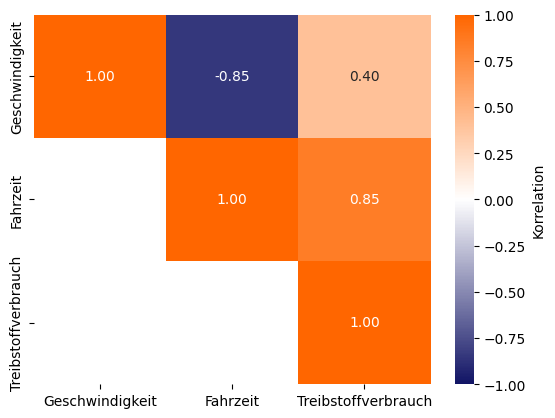
\includegraphics[width=\linewidth]{Thesis//bilder/corr-beispiel.png}
            \caption{Beispiel: Visualisierung Korrelationsanalyse}
            \label{fig:corr_analyse_bsp}
        \end{figure}
    \end{minipage}
        
     Die Spalten \textit{Durchschnittsgeschwindigkeit} und \textit{Fahrzeit} korrelieren im Gegenteil negativ. 
    Hier könnte also \textit{Fahrzeit} entfernt werden, da diese Information in der \textit{verbrauchten Treibstoffmenge} und \textit{Durchschnittsgeschwindigkeit} schon vorhanden ist.

    Bei der Korrelation gibt es keinen direkten Schwellenwert, woran optimal entschieden werden kann, ob eine zu hohe Korrelation besteht. Empirisch können aber Features identifiziert und bei der Feature-Auswahl entfernt werden.
    %QTODO
    
    \item \textbf{Datenkodierung:}  
    Viele Algorithmen des maschinellen Lernens können nur mit numerischen Daten arbeiten. 
    Bei einigen Algorithmen hängt dies von der Implementierung der verwendeten Softwarebibliothek ab.
    Bei den gewählten Implementierungen sind für \nameref{ref:impl_nn}, sowie \nameref{sec:impl_rf} eine Kodierung der kategorischen Daten notwendig. Wie diese Kodierung funktioniert, wird im nächsten \cref{ref:feat_encoding} erklärt.

\end{enumerate}


%Daten filtern, vielleicht nur mit validen valuations?

\subsection{Verarbeitung von nicht numerischen Daten}
\label{ref:feat_encoding}

Nicht numerische Daten stellen eine Herausforderung bei der Verarbeitung mit verschiedenen \gls{ml}-Modellen dar, da diese mathematische Operationen ausschließlich auf numerischen Werten ausführen können. 

Dies trifft auf neuronale Netze und die logistische Regression zu, hingegen beim Random Forest ist es implementierungsabhängig, ob die Eingabedaten kodiert werden müssen, da Random Forest abhängig von der Softwarebibliothek direkt Textdaten verarbeiten kann \cite{ydf2024, scikit-learn2024}.

Um diese Art von Daten verarbeiten zu können, müssen sie vorab in eine numerische Darstellung transformiert werden. In dieser Arbeit werden nur kategorische Textdaten verarbeitet, daher wurde sich auch nur auf Techniken bezogen, welche das Problem versuchen zu lösen.

\paragraph{Kategorische Daten}
Kategorische Daten bestehen aus diskreten Werten. Ein typisches Beispiel im Bereich einer Reederei sind Häfen, wie \enquote{Hamburg}, \enquote{Shanghai} oder \enquote{Rotterdam}, die als Start- oder Zielorte definiert sind. Zur Verarbeitung solcher Daten sind geeignete Techniken notwendig, da eine direkte Eingabe in das neuronale Netz nicht möglich ist. 

Wenn die kategorischen Daten eine natürliche Reihenfolge besitzen, kann jede Kategorie einfach durch einen Index ersetzt werden. 
Dies wird auch \enquote{ordinale Kodierung} genannt \cite{reusser2024tabularlearningencodingentity}.

Das Problem hierbei ist, dass die Kategorien nicht gezwungenermaßen vergleichbar sind, wie es die Indizes sind. 
Indizes führen eine künstliche numerische Ordnung ein. 
Wenn im Beispiel die Häfen in ihre Indizes $0, 1, 2$ transformiert werden, können Modelle diese Indizes miteinander vergleichen. 
Ein Modell würde \enquote{Hamburg} $0$ in der Ordnung kleiner als \enquote{Shanghai} $1$ einordnen. 
Dabei stehen diese Kategorien in keiner Ordnung. 
Um dieses Problem zu lösen, werden durch spezifische Methoden wie \enquote{One-Hot-Kodierung}, \enquote{Embedding} oder \enquote{Zielwert-Kodierung} die Indizes weiter umgeformt und die künstliche Reihenfolge entfernt.

\subparagraph{One-Hot-Kodierung}
\label{ref:t_one_hot}
Die \enquote{One-Hot-Kodierung} ist eine einfache und weitverbreitete Methode zur numerischen Repräsentation kategorischer Daten \cite{Goodfellow2016}. Jede Kategorie wird dabei in einen binären Vektor umgewandelt, dessen Länge der Anzahl der Kategorien entspricht. Für jede Kategorie ist genau ein Element des Vektors auf den Wert $1$ gesetzt, während alle anderen Elemente den Wert $0$ haben. Ein Beispiel hierfür ist in \cref{tab:one_hot_encoding_ports} dargestellt:

\begin{table}[H]
    \centering
    \begin{tabular}{clc}
        \hline\hline
         \thead{\textbf{Hafen}}  &\textbf{Index}& \textbf{One-Hot-Kodierung} \\ 
        \hline
         Hamburg  &$0$& [1, 0, 0] \\ 
         Shanghai  &$1$& [0, 1, 0] \\ 
         Rotterdam  &$2$& [0, 0, 1] \\
        \hline\hline
    \end{tabular}
    \caption{Beispiel für die One-Hot-Kodierung von Häfen}
    \label{tab:one_hot_encoding_ports}
\end{table}

Während die \enquote{One-Hot-Kodierung} für niedrige Kardinalitäten effizient ist, stößt es bei einer großen Anzahl an Kategorien an seine Grenzen. Der resultierende Vektorraum wächst linear mit der Anzahl der Kategorien (Kardinalität), was den Speicherbedarf und die Rechenzeit erheblich erhöht \cite{Bishop2006}.

\subparagraph{Embedding}
Eine effiziente Alternative für höhere Kardinalitäten bietet das \enquote{Embedding} \cite{9512057}. Dabei wird jeder Kategorie ein d-dimensionaler Vektor zugewiesen, dessen Werte während des Trainings gelernt werden. Diese komprimierte Darstellung erlaubt es, Ähnlichkeiten zwischen Kategorien zu erfassen. Im Fall von Häfen könnten Häfen derselben geografischen Region (z. B. „Hamburg“ und „Rotterdam“) im Vektorraum näher beieinander liegen als Häfen, die weit entfernt voneinander liegen (z. B. „Hamburg“ und „Shanghai“), wenn ihre logistischen oder geschäftlichen Beziehungen dies rechtfertigen.

Ein \enquote{Embedding} nutzt eine Gewichtungsmatrix $W \in \mathbf{R}^{N \times d}$, wobei $N$ die Anzahl der Kategorien und $d$ die festgelegte Embedding-Dimension ist. Die Transformation einer Kategorie mit Index $k$ in ihren entsprechenden Vektor erfolgt durch das Nachschlagen in der Gewichtungsmatrix. Diese Gewichtungsmatrix wird im Laufe des Trainings mittels der Rückpropagierung optimiert und bietet so eine lernfähige Repräsentation der Kategorien. Diese Technik kann also nur mit Algorithmen, welche mit der Rückpropagierung arbeiten, verwendet werden. Dies trifft hier nur auf die neuronalen Netze zu.

\begin{figure}[H]
    \centering
    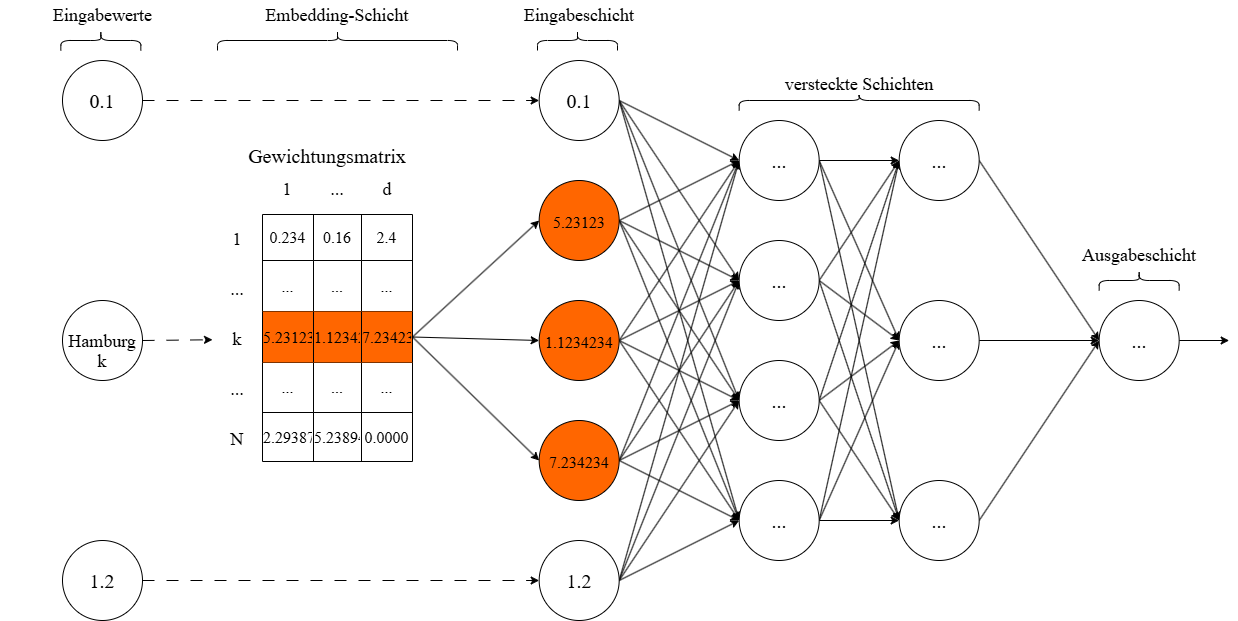
\includegraphics[width=0.9\linewidth]{Thesis//bilder/EmbeddingLayer.drawio.png}
    \caption
    {Visualisierung der Embedding-Schicht}
    \label{fig:embedding_layer_vis}
\end{figure}

In der Visualisierung ist eine Embedding-Dimension $d$ von $3$ gezeigt. Dabei soll verdeutlicht werden, dass wenn eine Kategorie, hier \enquote{Hamburg} mit Index $k$, als Eingabewert gegeben ist, in der Gewichtungsmatrix die entsprechende Zeile der Kategorie gelesen wird. 
Die Spalten-Werte werden dann als Eingabewert ins neutrale Netz übergeben. 
Sämtliche anderen numerischen Eingabewerte werden von dieser Schicht dabei nicht beeinflusst. 

\subparagraph{Zielwertkodierung}
Da Embedding nur mit neuronalen Netzen verwendet werden kann, wird eine effiziente Alternative für höhere Kardinalitäten benötigt. Dafür kann die Zielwertkodierung (auch Target Encoding) verwendet werden \cite{MicciBarreca2001}. 

Bei der Zielwert-Kodierung wird jeder Kategorie ein numerischer Wert zugewiesen, der auf den statistischen Eigenschaften der Zielvariable basiert. Die verwendete Methode ist die Mean-Encoding-Variante, bei der für jede Kategorie der mittlere Zielwert im Trainingsdatensatz berechnet wird.  

\pagebreak
Mathematisch ausgedrückt ist der Zielwert $T_k$ für eine Kategorie $k$ definiert als:
\[
    T_k = \frac{1}{N_k} \sum_{i=1}^{N_k} y_i
\]
wobei:
\begin{itemize}[noitemsep]
    \item $N_k$ die Anzahl der Beobachtungen in der Kategorie $k$ ist,
    \item $y_i$ der Zielwert für die $i$-te Beobachtung in dieser Kategorie ist.
\end{itemize}

Nehmen wir an, wir möchten Häfen als Feature kodieren, wobei das Ziel die Annahme ($y = 0$) oder Ablehnung ($y = 1$) einer Buchung ist. Die Zielwert-Kodierung würde dann für jeden Hafen den durchschnittlichen Anteil an angenommenen Buchungen berechnen:

\begin{table}[H]
    \centering
    \begin{tabular}{lcc|c}
        \hline\hline
        \thead{\textbf{Hafen}}& ...  & \textbf{Ziel} & \textbf{Zielwertkodierung (Anteil Ablehnung)} \\ 
        \hline
        Hamburg  & ... & 0 & \multirow{2}{*}{0}  \\ 
        Hamburg  & ... & 0 &   \\ 
        \hline
        Shanghai & ... & 0 & \multirow{3}{*}{0.6667}  \\
        Shanghai & ... & 1 &   \\
        Shanghai & ... & 1 &   \\ 
        \hline
        Rotterdam & ... & 1 & \multirow{2}{*}{0.5}  \\
        Rotterdam & ... & 0 &   \\
        \hline\hline
    \end{tabular}
    \caption{Beispiel für Zielwert-Kodierung von Häfen}
    \label{tab:target_encoding_ports}
\end{table}

Nach der Kodierung ersetzt der berechnete Mittelwert die ursprüngliche Kategorie. 

%Todo: Wie wird d bestimmt. -> Vielleicht wie wird d bestimmt
%Todo: Vielleicht mehr daruf eingehen, wie die werte optimiert werden
%\todo{J: Wie kommen die Werte in der Tabelle zustande und wie wird die konstante d gewählt?}
\paragraph{Wahl der Kodierung}
Abhängig von der verwendeten Softwarebibliothek muss vorerst überhaupt entschieden werden, ob eine Kodierung notwendig ist. 
Wenn eine Kodierung notwendig ist, hängt von der Kardinalität der Kategorien ab, ob eine \enquote{One-Hot-Kodierung} infrage kommt. 
Während die \enquote{One-Hot-Kodierung} einfach zu implementieren ist, bieten \enquote{Embedding} und \enquote{Zielwertkodierung} signifikante Vorteile bei höheren Kardinalitäten. 
Der Implementierungsaufwand der Ansätze ist von der gewählten Softwarebibliothek abhängig, daher werden in dieser Arbeit alle Ansätze verwendet. 

%\todo{IW: Frage Implementations übernahem}
%Hier sprechen Sie einen Punkt an, den ich selbst in der Praxis nie erfahren habe und der bisher nicht von meinen Absolventen thematisiert wurde.
%Meine Frage dazu: Müssen sich alle Anwender tatsächlich selbst um die numerische Codierung der nichtnumerischen Daten kümmern, oder gibt es da auch Hilfen durch die entsprechenden Softwarebibliotheken, wo Sie als Werte durchaus nichtnumerische
%Daten angeben können und mit diesen direkt die Netzwerke trainieren können?
%Sie müssen sich ja auch nicht um die Details der Backpropagation kümmern. Das lösen die entsprechenden Bibliotheken alleine, wobei mir unklar geblieben ist, ob die von Ihnen gewählte das tatsächlich macht.

